\subsection{Allgemein}
\begin{itemize}
\item zur Nutzung nur die \hyperref[scdc.h]{scdc.h} einbinden (Die anderen Bibliotheken sind eher für den internen Gebrauch gedacht)
\item SCDC kann statisch gebunden werden. Lib dazu ist libscdc.a.
\item Pfad eines Ortes mit Service scdc+<protokoll>://<host>/<dataprovidername>/<dataset>\\
      BSP: je nach Methode:
      \begin{itemize}
      \item[--] {\color{darkgreen}direct:} direkte Funktionsaufrufe, \\
                URL: scdc:/<path>
      \item[--] {\color{darkgreen}uds:} Interprozesskommunikation mit UNIX Domain Socket, \\
                URL: scdc+uds://<socketname>/<path>
      \item[--] {\color{darkgreen}tcp:} Netzwerkkommunikation mit TCP, \\
                URL: scdc+tcp://<hostname>/<path>
      \item[--] {\color{darkgreen}mpi:} HPC-kommunikation mit MPI,\\
                URL: scdc+mpi://<world/comm/port/publ>:<rank>/<path>
      \end{itemize}
      Bezeichnungen festlegen in Funktionen:\\
      Protokoll >> \hyperref[scdc_nodeport_open]{Nodeport} :// Dataprovidername >> \hyperref[scdc_dataprov_open]{Datenprovider} / 
      Datensetbezeichnung(path) >> \hyperref[scdc_dataset_open]{Datenset}
\item Datensätze sind vor allem gedacht, um mehrere Kommandos auf Daten auszuführen. Datenprovider dagegen können mehrere Datensätze beinhalten, können aber auch so Daten speichern. Sie können die eine CMD-Funktion von den Datensätzen \texttt{scdc\_dataprov\_hook\_dataset\_cmd\_f} benutzen, um bestimmte Berechnungen auf den meistens mitgelieferten Daten auszuführen, wenn keine Datensätze vorhanden. (Nur wenn Datensätze anzulegen sich nicht lohnt.)
\item Datenprovider und Datensätze haben über die CMD-Funktion immer die Parameter Input und Output für Datentransfer
\item Für Input und Output können nur einfache zusammenhängende Arrays übertragen werden.
\end{itemize}

\subsection{Server}
Stellt den Dienst und den Datenprovider bereit.
Datasets auf denen der Client Befehle ausführt liegen dort bei diesem.
Datenprovider und Nodeports müssen konfiguriert werden.
Nodeports dienen als die Serverschnittstelle und öffnen diese und binden sich an einen Port.

\begin{enumerate}
	\item SCDC Initialisieren mit \hyperref[scdc_init]{scdc\_init(SCDC\_INIT\_DEFAULT)}
	\item Anlegen der Variable vom Typ \Hhref{scdc_dataprov_hook_t} BSP: \texttt{scdc\_dataprov\_hook\_t hook\_functions}.
	\item Implementieren der Hookfunktionen siehe Kapitel \ref{scdc_dataprov_hook_open_f}
	\item Vermerken der Funktionen in der Variable vom Typ \Hhref{scdc_dataprov_hook_t}. Alle nicht benötigten Funktionen sind mit 0 einzutragen.
	\item Datenprovider eröffnen mit \hyperref[scdc_dataprov_open]{scdc\_dataprov\_open(\qqq{Providername}, \qqq{hook}, \&hook\_functions)}.
	\item Nodeport öffnen \hyperref[scdc_nodeport_open]{np\_tcp = scdc\_nodeport\_open(\qqq{<protokoll>:<optionen>}, optionswerte)}, damit der Server nach außen auf einem Port hört
	\item Server starten \hyperref[scdc_nodeport_start]{scdc\_nodeport\_start(np\_tcp, SCDC\_NODEPORT\_START\_LOOP\_UNTIL\_CANCEL)} und Anfragen entgegennehmen lassen.
	\item Server läuft und arbeitet
	\item Beenden: 
	\item Nodeport stoppen und Verbindung schließen \hyperref[scdc_nodeport_stop]{scdc\_nodeport\_stop(np\_tcp)}
	\item Nodeport schließen \hyperref[scdc_nodeport_close]{scdc\_nodeport\_close(np\_tcp)}
	\item Datenprovider schließen \hyperref[scdc_dataprov_close]{scdc\_dataprov\_close(dp\_hook)}
	\item SCDC wieder schließen mit \hyperref[scdc_release]{scdc\_release()}
\end{enumerate}



\subsection{Client}
Öffnet die Verbindung zum Dataset auf Server xy und führt auf dem Datensatz Kommandos cmd aus.
Der Datensatz kann hoch und runter geladen werden.
\begin{enumerate}
	\item SCDC Initialisieren mit \hyperref[scdc_init]{scdc\_init(SCDC\_INIT\_DEFAULT)}
	\item Datensatz mit der Adresse \texttt{uri} öffnen: \texttt{dataset = \hyperref[scdc_dataset_open]{scdc\_dataset\_open(uri)}}
	\item Input-Objekt vom Typ \hyperref[scdc_dataset_input_t]{scdc\_dataset\_input\_t} anlegen und vorbereiten. (Variable anlegen, mit \hyperref[scdc_dataset_input_unset]{scdc\_dataset\_input\_unset()} initialisieren (Elemente der Struktur auf definierte Nullwerte) und benötigte Werte in der Struktur setzen, um Daten zum Server zu übermitteln)
	\item Output-Objekt vom Typ \hyperref[scdc_dataset_output_t]{scdc\_dataset\_output\_t} vorbereiten. (Variable anlegen, mit \hyperref[scdc_dataset_output_unset]{scdc\_dataset\_output\_unset()} initialisieren (Elemente der Struktur auf definierte Nullwerte)  und benötigte Werte in der Struktur setzen, um Daten vom Server zurückzubekommen)
	\item Kommando auf dem Datensatz auf dem Server ausführen. Server führt Berechnungen durch nimmt dabei die Daten vom Input-Objekt input entgegen\\
	      Aufruf: \texttt{ \hyperref[scdc_dataset_cmd]{scdc\_dataset\_cmd(dataset, \qqq{Kommando}, \&input, \&output)} }
	\item Entnehmen der vom Server zurückgelieferten Daten aus dem Output-Objekt output
	\item Datensatz schließen mit \hyperref[scdc_dataset_close]{scdc\_dataset\_close(dataset)}
	\item SCDC wieder schließen mit \hyperref[scdc_release]{scdc\_release()}
\end{enumerate}


\begin{center}
 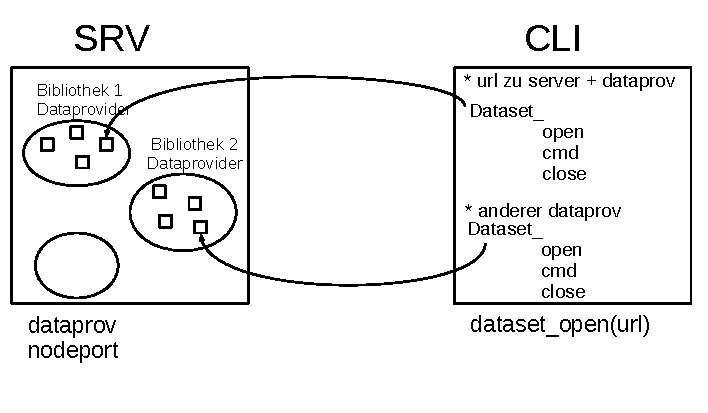
\includegraphics[width=0.7\textwidth]{img/srvcli}
\end{center}
